\documentclass[letterpaper,10pt,compsoc,draftclsnofoot,onecolumn]{IEEEtran}

\usepackage[margin=0.75in]{geometry}
\usepackage[parfill]{parskip}
\usepackage[singlespacing]{setspace}

\usepackage{array}
\usepackage{beramono}
\usepackage{caption}
\usepackage{color}
\usepackage{cite}
\usepackage{graphicx}
\usepackage{helvet}
\usepackage{hyperref}
\usepackage{listings}
\usepackage{tabularx}

\title{
	\fontfamily{phv}\fontsize{36pt}{36pt}\fontseries{bx}\selectfont{
        AMD Hammer Architecture
        \\\vspace{1em}
        VS
        \\\vspace{1em}
        Intel Core2 Architecture
	}
}
\author{}
\date{\today}
\hypersetup{
	colorlinks = true,
    citecolor = black,
	urlcolor = black,
	pdfauthor = {Songjian Luan},
	pdfkeywords = {CS472 ``Computer Architecture"},
	pdftitle = {CS472 Final Project},
	pdfsubject = {CS472 AMD Hammer vs Intel Architecture},
	pdfpagemode = UseNone
}

\begin{document}
\pagenumbering{gobble}
\begin{titlepage}
\begin{minipage}{1.0\textwidth}
\centering{OREGON STATE UNIVERSITY
\\\vspace{1em}
CS472 - Final Paper}
\end{minipage}
\vfill
{\let\newpage\relax\maketitle}
\vfill
\begin{minipage}{1.0\textwidth}
\centering{\textbf{Instructor:} D. Kevin McGrath\\\vspace{1em}\textbf{Email:} dmcgrath@eecs.oregonstate.edu}
\end{minipage}
\vfill
\begin{minipage}{1.0\textwidth}
\centering{\textbf{Name:} Luan Songjian\\\vspace{1em}\textbf{Email:} luans@oregonstate.edu}
\end{minipage}
\vfill
\begin{abstract}
\noindent In this final paper, I choose the AMD Hammer architecture to compare with the Intel Core 2 architecture. These two corporations are the arch rival because they are the maximum producers and vendors  in the world and have individual advantages in the CPU market. According to my past experience and source materials found online, both architectures can be contrasted based on their history and product’s design. Therefore, I am a little interested in learning and understand both architectures through following attributes.
\end{abstract}
\end{titlepage}
\pagenumbering{arabic}

\section{Introduction}
\subsection{History}
\subsubsection{Intel Core 2}
The Intel as the biggest producer and vendor of CPU in the world has created so many legend CPUs. The Core 2 is a brand encompassing a range of Intel's consumer x86-64 with single, dual, and quad core microprocessors based on the core micro architecture. The CPU with single core like Pentium series and the dual core models are single-die; however, the quad core models cannot be packaged in a multi-ship module for each containing two cores\cite{pdf_intel_core}. The Pentium brand was relegated by the introduction of Core 2 to the mid-range market. Also, this series had reunified laptop and desktop CPU lines, which previously had been divided into the Pentium 4, Pentium D, and Pentium M brands.

On the July 27 2006, the Core 2 brand was introduced to comprise the single core (Solo),  dual core (Duo), and quad core (Quad) in 2007. In addition, the Extreme series with dual and quad core CPUs for enthusiasts is the sub brand of Intel Core 2 processors. This series CPU mainly is placed in advanced products, comparing to the Duo and Quad.

\subsubsection{AMD Hammer}
The AMD is another famous and big scale of cooperation which product and supply CPU. It owes a similar debt to the K7 core and the main architecture by this company has staked on  its processor business because of the Athlon processor created in 1999. The CPU with P6 architecture like the Athlon line and the K7 architecture CPU have become successful performance story in commercial market. The K7 CPU vaulted AMD to the top of the performance ladder,  which enable this company to shake the leadership of performance by Intel and occupy some market shares. The K7 CPU also can hang on to what will lead for some important stretches of time.

However, given the Athlon's continuous performance scaling, it does not have any surprise when AMD hatched the idea of bringing x86 into the x86\_64 series. In fact, both architectures are decided to build on the K7 architecture, instead of creating a completely new design from the scratch\cite{inside_amd_64}. But, for a few significant changes and a large number of tweaks. The hammer architecture, so-called K8, brings both the K7 architecture and the x86 instruction set into the future. Actually, the K8 core is very similar to the K7 due to the most radical changes in AMD64 instructions and an on-chip memory controller. This memory controller can drastically reduce memory latency and enable most of the performance to gain from K7 to K8.

\subsection{Family}
\begin{table}[!bhpt]
\captionsetup{justification=centering, aboveskip=2em, belowskip=0em}
\begin{tabularx}{\textwidth}{m{1in}m{2in}m{2in}m{1in}}
\textbf{Processor} & \textbf{Platform} & \textbf{Model} & \textbf{Socket}
\\
Core 2 Duo & Desktop & E4xxx, E6xxx, E7xxx, E8xxx & LGA775, LGA771
\\
Core 2 Quad & Desktop & Q6xxx, Q8xxx, Q9xxx & LGA775
\\
Core 2 Extreme & Desktop & X6xxx & LGA775, LGA771
\\
Sempron & Desktop & 2xxx+, 3xxx+ & A, 754, 939, AM2, S1, AM3, AM1
\\
Athlon 64($\times$2) & Desktop & 3xxx+, 4xxx+, 5xxx+, 6xxx+, 7xxx+ & 754, 939, 940, AM2, AM2+
\\
Opteron & Server and Workstation &  & 939, 940, AM2, AM2+, AM3, AM3+, F, C32, G34
\\
Turion 64($\times2$) & Mobile &  &
\end{tabularx}
\caption{Intel Core 2 and AMD Hammer Family}
\end{table}
\clearpage
\subsection{Architecture}
\begin{figure*}[!bhpt]
\captionsetup{justification=centering, aboveskip=2em, belowskip=0em}
\begin{minipage}{0.5\textwidth}
\centering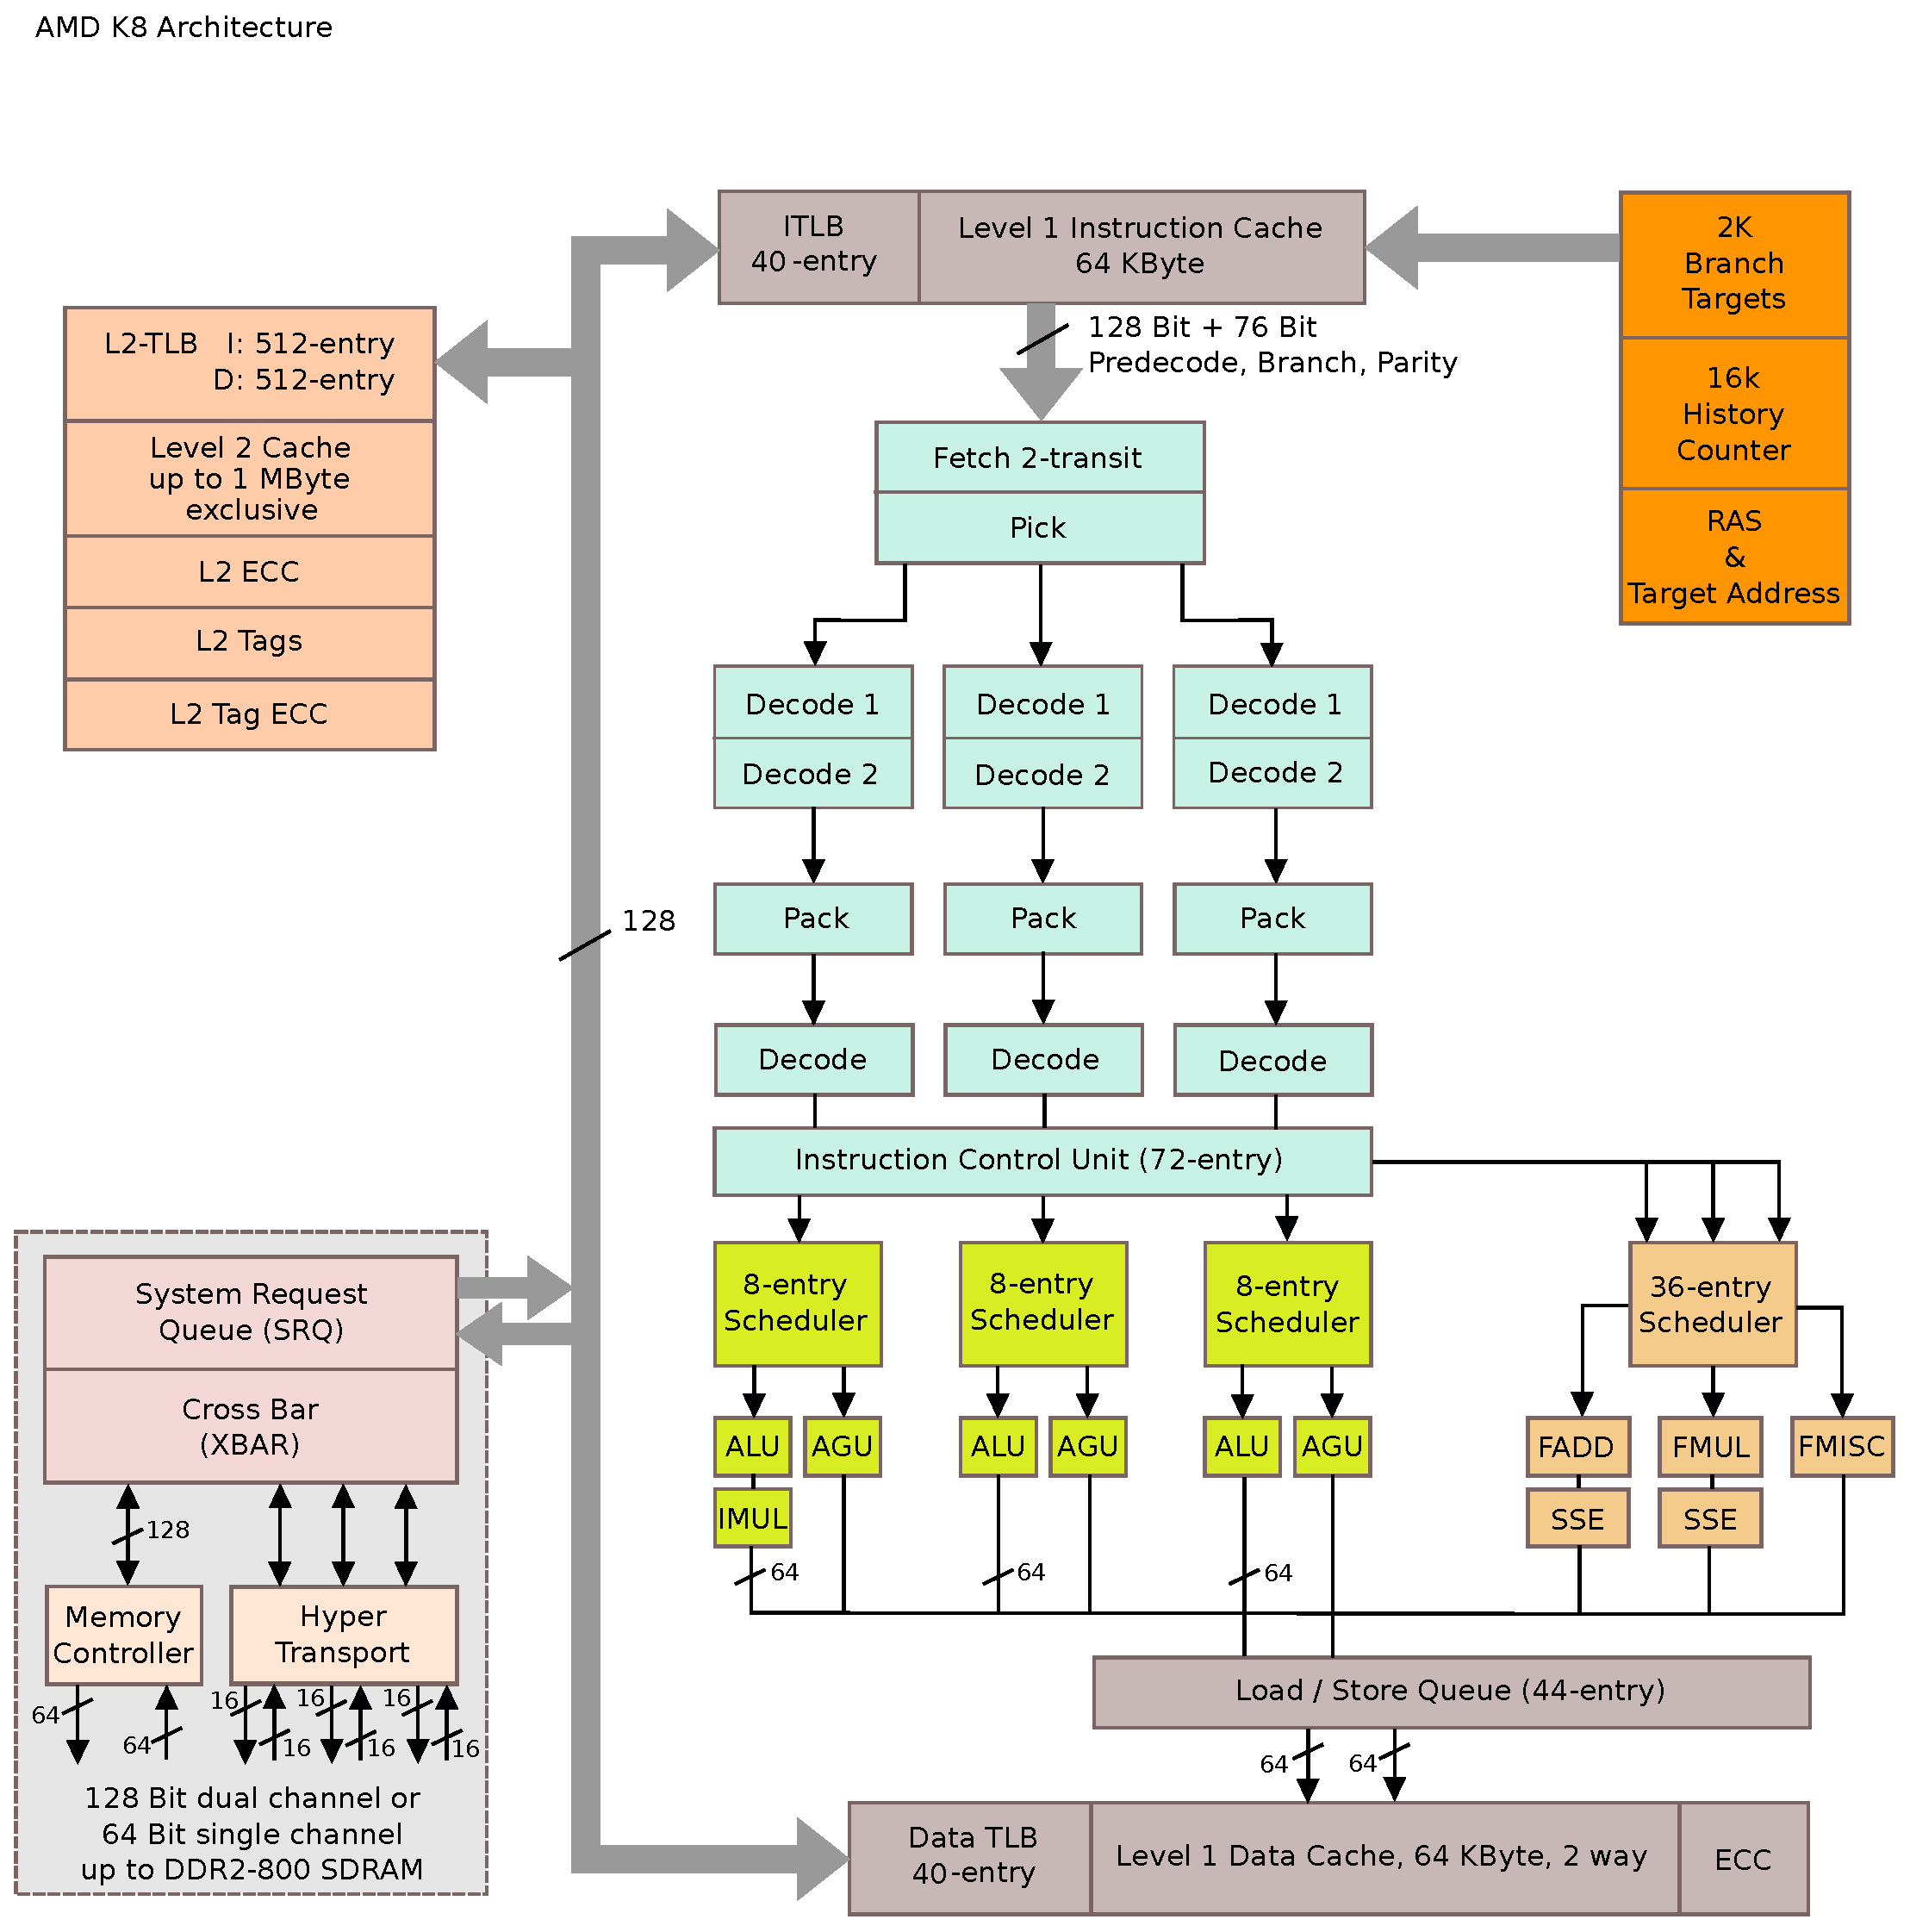
\includegraphics[scale=0.2]{figures/AMD_K8}
\caption{AMD K8 Architecture\cite{amd_k8}}
\label{fig:K8}
\end{minipage}
%
\captionsetup{justification=centering, aboveskip=2em, belowskip=0em}
\begin{minipage}{0.5\textwidth}
\centering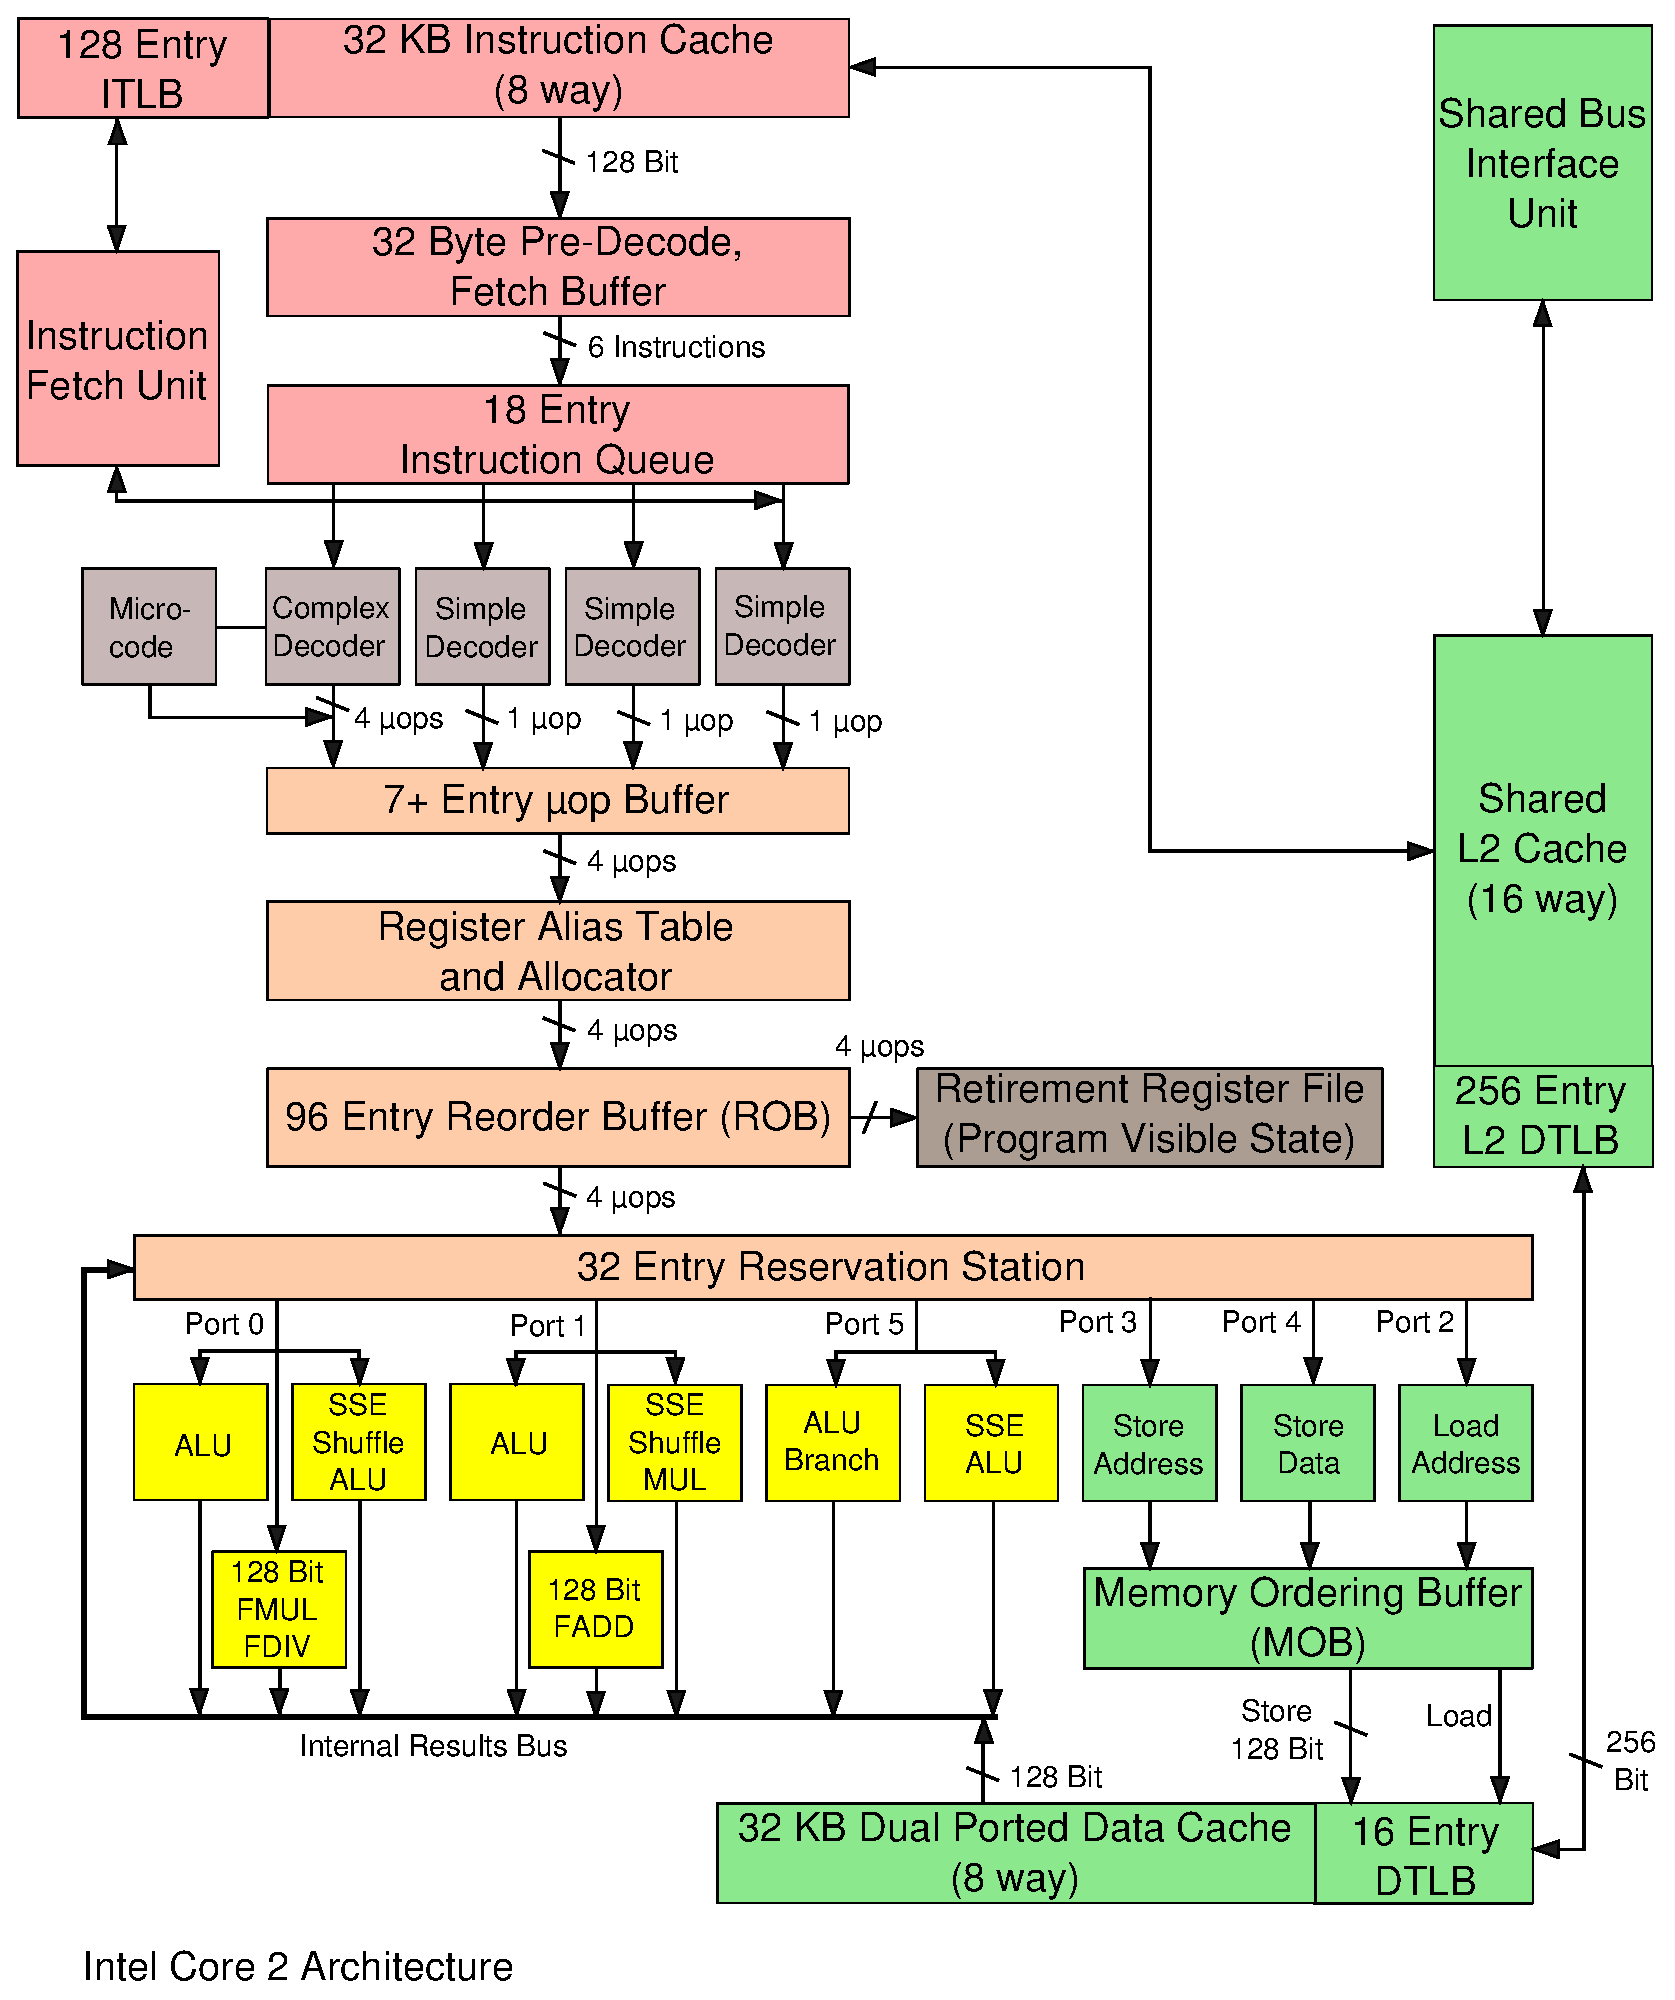
\includegraphics[scale=0.23]{figures/Intel_Core2}
\caption{Intel Core2 Architecture\cite{intel_core2}}
\label{fig:K8}
\end{minipage}
\end{figure*}

\section{Instruction Set Design}
\subsection{Type}
The Intel Core 2 uses CISC but the Hammer is a RISC machine without ideas of x86 instructions or machine state. The AMD Hammer has been beyond the first few stages of the pipeline.

\subsection{Address}
The AMD Hammer has nine execution units, like the Athlon and Itanium coincidentally. Those nine execution units are divided into three integer units which are arithmetic units, logic units, and aka ALUs. In addition, there are three address-generation units (AGUs) and three floating-point units. In this point, it is very similar to Athlon and any architecture of K6 or before. Although Hammer has nine execution units, it is very difficult to explain why it can accomplish the same amount of work per cycle to the K6 processors or before. Otherwise, the AMD Hammer has three address-generation units which do not exist in K6 processors or before, which do not really contribute to forward progress.

\subsection{Support}
As shown in the table below, Intel Core 2 and AMD Hammer architectures have several common instruction set supported, but both have individual or special instruction set supported.

\begin{table}[!bhpt]
\captionsetup{justification=centering, aboveskip=2em, belowskip=0em}
\begin{tabularx}{\textwidth}{m{0.3\textwidth}m{0.3\textwidth}m{0.3\textwidth}}
 & \textbf{Intel Core 2} & \textbf{AMD Hammer}
\\
MMX & yes & yes
\\
SSE & yes & yes
\\
SSE2 & yes & yes
\\
SSE3 & yes & yes
\\
EM64T & yes & no
\\
3DNOW+ & no & yes
\\
x86\_64 & no & yes
\end{tabularx}
\caption{Intel Core 2 and AMD Hammer Instruction Set}
\end{table}

\subsubsection{SSE2 Instruction Set Support}
Intel introduced the SSE2 instruction set for single-instruction and multiple-data in SIMD calculations with the Pentium 4. However, the SSE2 instructions set allows for SIMD instructions set operations on 128-bit IEEE double-precision floating-point datatypes\cite{amd_athlon_64}. Therefore, it is very useful in tasks, such as 3D rendering, graphics drivers, gaming, and media encoding. The previous Athlon chips have supported SIMD instruction set extensions for both integer in MMX instruction set and single-precision floating-point in operations of SSE and 3DNow! Instruction sets. However, they have been missing SSE2 impacted by the SIMD instruction set on x86. The Hammer architecture can keep the advantage of applications optimized for SSE2 instruction set. It makes more competitive with the Intel Core 2.

\subsubsection{AMD64 Instruction Set Support}
The AMD64 (x86\_64) has been designed by the AMD which own instruction set of extensions to the x86 instruction set architecture, or ISA. The new AMD64 instruction set architecture is not a radical departure, but it allows for 64-bit addressing adds some extra registers in x86 ISA. Therefore, the AMD is ready to move to 64 bits accomplishes in several things.

First, this instruction set can eliminate the barrier due to 4GB addressable memory in the 32-bit operating systems. Although the 4GB limitation is very universal in the Hammer time, but the 4GB as an upper limitation can become a nasty constraint on common desktop systems in those following years. Second, by adding 32-bit extensions to the x86 ISA, the AMD has created an evolutionary alternative to Intel's Itanium chips, which break with the industry-standard x86 software infrastructure\cite{amd_athlon_64}. Naturally, the code also will have to be recompiled for the AMD64 instruction set. But this instruction set is so familiar enough that some compilers should be relatively painless. Finally, for the AMD64 additional registers, they are present in Hammer and promise better performance on recompiled code. Addressing memory in 64-bit chunks will not necessarily improve performance by itself. Otherwise, there are eight new 64-bit integer registers and eight new 128-bit SSE/SSE2 registers for Hammer to help.

\section{Datapath Design}
\subsection{Register}
The AMD Hammer architecture is a typical 64-bit architecture invented by some new 64-bit instructions. There is a whole new set of floating-point operations that use a new flat FP register file of sixteen 128-bit registers\cite{hammer_amd_arch}.The floating-point capabilities of the Intel Core 2 architecture were the low point of an already awkward architecture.

The Hammer also provides mixed code size compatibility which is the same way the 386 did. Any existing instruction in Hammer architecture can be prefixed with the one-byte REX pseudo-instruction\cite{amd_athlon_64}. In addition, this byte tells the decoder that the operands in this instruction should be interpreted as 64-bit quantities. The Hammer architecture does not expose parallelism or anything else to the compiler. It is just another turbocharged x86 with really fast at x86 code in architecture. New Hammer code can access all the new registers, and even treat them as a flat register file. But it cannot break free of the x86 instruction set. In general, the problem is not the binary encoding of x86 instructions. The AMD and other processor productors have shown that they can build blazing fast x86 chips with RISC like internals, and even with the fundamental x86 handicap. It is possible way for x86 architecture to overcome in the parallel nature.

\subsection{Cycle}
The fetch phase in Hammer architecture has been broken up into two stages which are compared to the Athlon's single-cycle fetch stage. This two-cycle fetch is integrated in many processors because this kind of fetch way can help to decouple the clock speed from L1 cache access latency.

However, the Hammer architecture is moved from these sixteen bytes to a 32-byte buffer, which can append the new 16-byte group fetched onto the previous 16-byte fetched group. The processor can scan this 32-byte batch of instructions and then pick out instruction boundaries after aligning the instructions\cite{inside_amd_64}. Finally, instructions are sorted into one of two types that can be decoded by decoder directly. Furthermore, those also must be decoded by the microcode engine and then aligned to the decode stage sent.

Like the Athlon which is a typical Hammer processor, the Hammer architecture can do both the scanning and aligning in one-cycle fetch. That is because the pre-decoded instruction boundary data is cheated to be added, when the instructions were fetched into the L1 cache\cite{pdf_amd_k8}.

\subsection{Pipeline}
The Hammer's decoding hardware is quite similar to the Athlon. Both architectures have two types in decode hardware: one is the so-called direct Fastpath decoder and another is the microcode engine. Both of decoders will translate x86 instructions into an internal instruction set, like the RISC format. That is much easier for the processors to execute, manage, and schedule cores. In addition, the Hammer architecture has a longer pipeline than Itanium at 12 stages\cite{pdf_amd_k8}. It should not be surprised that most of small differences are spent decoding x86 instructions and converting them to more digestible ROPs.

The Hammer architecture can decode up to three x86 instructions and dispatch up to 9 ROPs per cycle. Assuming the best case mapping to one of nine execution units in Hammer. Most ROPs execute directly in hardware, but even after conversion because of the perversion by some x86 operations. These are trapped and emulated by routines in Hammer's micro-ROM, just like Athlon.

In Hammer architecture, the executions of fetch and decode are the first two stages in the classic RISC four-stage pipeline\cite{redhat_amd}. The fetch phase can be divided into two individual pipeline stages and the decode phase can be used to cover either two, four, or more stages. It depends on which stages will be decided to include. Aside from the acts of fetching and decoding instructions, the most important thing is to takes place over the two phases by branch prediction. Branches in the code stream can be identified and predicted in a processor pipeline as soon as possible. Therefore, the front-end of processors can be quickly filled by instructions from the new location in the code.

\section{Memory Subsystem}
\subsection{Limits}
In this section, I am interested in comparing the real-life performance of the Core 2 Duo platform to the Athlon 64×2 platform, which is a legend AMD Hammer processor. Because they use different methods to placing the memory controller, the comparison of the Core 2 Duo and the Athlon 64×2 has an internal DDR2 SDRAM controller, which will integrated right into the CPU core\cite{pdf_amd_k8}. Moreover, both integrated controller provide a very high memory bandwidth which is the bit-rate of information capacity expressed in bits per second. For example, the Athlon 64×2 can handle dual channel DDR2 800 so that have equivalent memory bandwidth to a 1600 MHz FSB provided.

Otherwise, the substantial advantage over the Core 2 Duo architecture is not to be considered and the speed of data transfers between the processor and memory is limited by the bandwidth of the FSB. As a consequence, this design will enhance 40\% efficiency in DDR2 800 SDRAM memory subsystem and the new Intel CPU will enhance 55\% to 60\% efficiency on the Athlon 64 X2 platform\cite{hammer_amd_arch}.

\subsection{Cache}
The cache subsystem in the Hammer is not changed too much from the Athlon. As value shown in table below, The L1 cache has data cache and instruction cache. Both caches have 64KB as the default size. But the data cache is 2-way set associative with low hit rate as is the instruction cache. Similarly, the Core 2 Duo, Core 2 Quad, and Core 2 Extreme have the same 64KB+64KB as the default size of L1 data cache and instruction cache.

The L2 cache is another cache subsystem. However, the time around AMD is only committing to a maximum of 1MB for the L2 cache\cite{inside_amd_64}. For example, the release of the Athlon processor was hinting at the possibility of L2 cache sizes up to 8MB. When we know that the Athlon with 1MB L2 cache size based on the nixed Mustang\cite{inside_amd_64} core were produced, nothing ever made it to market did not do anything with a larger L2 cache. As shown in the table below, all AMD Hammer processors have 256KB, 512KB, 1024KB, or more as the default L2 cache size. For how to assign a proper size for the L2 cache, it will depend on product’s requirements. But, there is a huge difference in Core 2 processor. For the Duo, Quad, and Extreme, they are assigned a size for L2 cache between 1MB and 12MB. That is the reason why Intel Core 2 processors are more powerful than the AMD Hammer series of processors.

\begin{table}[!bhpt]
\captionsetup{justification=centering, aboveskip=2em, belowskip=0em}
\begin{tabularx}{\textwidth}{m{0.25\textwidth}m{0.25\textwidth}m{0.25\textwidth}m{0.25\textwidth}}
 & \textbf{AMD Hammer} & \textbf{Intel Core 2} &
\\
Athlon64($\times$2) & L1: 64KB+64KB L2: 256KB, 512 KB, 1024KB & L1: 64KB+64KB L2: 1MB-12MB & Duo
\\
Sempron & L1: 64KB+64KB L2: 128KB, 256KB, 512KB & L1: 64KB+64KB L2: 1MB-12MB & Quad
\\
Opteron & L1: 64KB+64KB L2: 1024KB & L1: 64KB+64KB L2: 1MB-12MB & Extreme
\\
Turion 64 ($\times$2) & L1: 64KB+64KB L2: 512KB or 1024KB & &
\end{tabularx}
\caption{Hammer and Core 2 Cache Size Table}
\end{table}

The AMD Hammer architecture has two small but noteworthy advantages. The first advantage is that it has two L1 cache with 64KB for each. The main purpose of this design only is a small advantage as an 8-way 32 KB cache, which is designed in current Core i processors now. It will have a hit rate close to the 2-way 64 KB cache. The second advantage is very important because it is the on die memory controller, which lowers the latency to the memory considerably\cite{pdf_amd_mem}. However, it is very similar to the lower clock speeds of the Core processors like the NetBurst and the faster FSB also lower latency significantly. With some tested data, the latency advantage of the Athlon 64×2 will shrink to only 15\% to 20\%. For comparison, the memory subsystem of the Core 2 Duo was almost twice as slow as the Athlon 64$\times$2, almost like 80 to 90 ns VS 45 to 50 ns.

However, both small advantages are likely negated by all the other memory subsystem metrics because the Core processors have much bigger caches and smarter prefetching than the competition. Otherwise, the Core architecture L1 caches have double 64KB sizes and can deliver about twice as much bandwidth. For instance, the L2 cache has about 2.5 times faster than the Athlon 64 or Opteron processors in AMD Hammer architecture. There are quite a few explanations to introduce why Core 2 Duo processors may put forth specific requirements to the memory subsystem to achieve maximum performance. First, these Intel Core 2 processors are compatible with the same LGA 775 platforms which are minor variations in electric characteristics. The LGA 775 platform has long and deep study processors from the Pentium 4 and D families in some early processors. But as a matter of fact, the Core 2 Duo has a dramatically different micro architecture which is the main reason for its different way of working with system RAM\cite{pdf_intel_duo}.

Otherwise, we will see 512KB parts for the performance desktop and entry-level workstation segments, and 1MB parts for the high end servers. Considering AMD stressing of its stellar performance while dealing with large workloads, if AMD Hammer would eventually create a Duron-like version in the Hammer processor, then it would be feasible for a processor like to only have a 256KB L2 cache.

\subsection{Data Interaction}
If the Hammer processors have the L2 cache the 16-way set like the Thunderbird/Palomino cores, it will assure us that the L2 cache is designed independently for the Athlon that will make any similarities between the two purely. Because it possibly is the right way to do this. When the AMD Hammer confirms that the L2 cache will  be solved more efficiently, we will have to get confirmation from what the L2 core interface has been widened\cite{pdf_intel_duo}, particularly in the currently crippling 64-bit data path.

First of all, the Intel Core 2 innovative Duo design with a shared L2 cache can free the front-side bus and the memory bus from data transferring required to maintain data coherency in separated L2 caches. For example, the Pentium D  processors used to to exchange data between the execution cores and buses of the front-side and memory, whereas the Core 2 Duo achieves this by means of its shared L2 cache alone\cite{pdf_intel_core}. As a consequence, the Core 2 Duo can use the CPU-memory link to do more effect and free it from auxiliary data transfers.

In addition, The Core 2 Duo systems have a positive effect on memory performance which has the increased frequency of the Quad Pumped Bus\cite{pdf_amd_mem} and connects the processor to the North Bridge chipset. For instance, the resulting frequency in this bus has been changed to 1067MHz now, which provides a bandwidth of 8.5GB/s. This change also explains that the Core 2 Duo platforms have an opportunity to fully utilize the bandwidth provided by a dual channel DDR2 533 SDRAM. Moreover, it is a good chance to install even higher frequency modules to reduce memory access latencies additionally.

Lastly, Although the Core 2 Duo from Intel access memory through the same memory controller has integrated into the North Bridge chipset, the choice of the processor affects the result greatly. Additionally, the Core 2 Duo processors can ensure a 10\% higher memory bandwidth and much lower data access latency with 20\% to 40\%\cite{pdf_amd_mem}, depending on the data prefetch algorithms. The Core 2 Duo is an obviously superior to use the memory subsystem efficiently.

Generally, as for the memory latency parameter, the Core 2 Duo platform is capable of achieving lower memory latency than the Athlon 64×2 system. This result also is decided by the data prefetch algorithms within the Core microarchitecture. Those algorithms prove to be very helpful in many cases. So, for an external memory controller, the Core 2 processors have high performance in applications sensitive to memory speed than the AMD Hammer processors .

\subsection{Virtual Memory Supported}
The straightforward approach of AMD Hammer to 64-bit computing builds upon the x86 instruction set, which is mostly proven and widely supported technologies. However, the AMD x86-64 technology is designed to support some applications with addressing a large amounts of physical and virtual memory. For example, high-performance servers, database management systems, and CAD tools\cite{pdf_amd_mem}. The Hammer processors are typically integrated AMD x86-64 technology into current computing and supporting environment. Additionally, it is designed to deploy high-performance 64-bit capable systems for enterprises, which build on invested in 32-bit software.

There are two way to realize that. First, the Hammer lowers memory latencies can be used to call the large workload TLBs. In this way, this method can make processors properly understand how to translate look-aside buffer works. Fortunately, the virtual memory in Hammer architecture can support this method. Second, when a processor performs a memory access, it must translate the specific logical address in the memory access instruction at first and then to a physical address\cite{pdf_amd_mem}. This physical address must be able to tell the processor requiring data located in RAM. Because the address translation process involves accessing a kind of data structure like the page table to be stored in main memory, a single memory access theoretically involves to either fetch proper the Page Table Entry (PTE) or actually read or write the data\cite{pdf_amd_mem}.

Otherwise, because it can work on only one x86 instruction at a time, the microcode decoder has much less decode bandwidth than the Fastpath decoder. Therefore, the Hammer architecture has beefed up the Fastpath decoder to translate a wider range of instructions. Some instructions  in Athlon are translated by using the microcode engine, but the instructions in Hammer translated directly. That is why the floating-point and SSE instructions are so important that they have been moved to Fastpath on the Hammer.

In order to prevent each memory access from requiring a page table access, The translation speeds up the process of address translation by caching the results of previous address translations. When the processor has to perform an address translation, it must checks the TLB according to translation had been performed recently. If so, then it can get the physical address directly from the TLB, instead of fetching the proper TLB from the memory and an address calculated. Thus, the TLB cuts down on average memory access latencies by reducing some memory accesses requiring an extra memory access to be completed.

\begin{figure*}[!bhpt]
\captionsetup{justification=centering, aboveskip=2em, belowskip=0em}
\begin{minipage}{1.0\textwidth}
\centering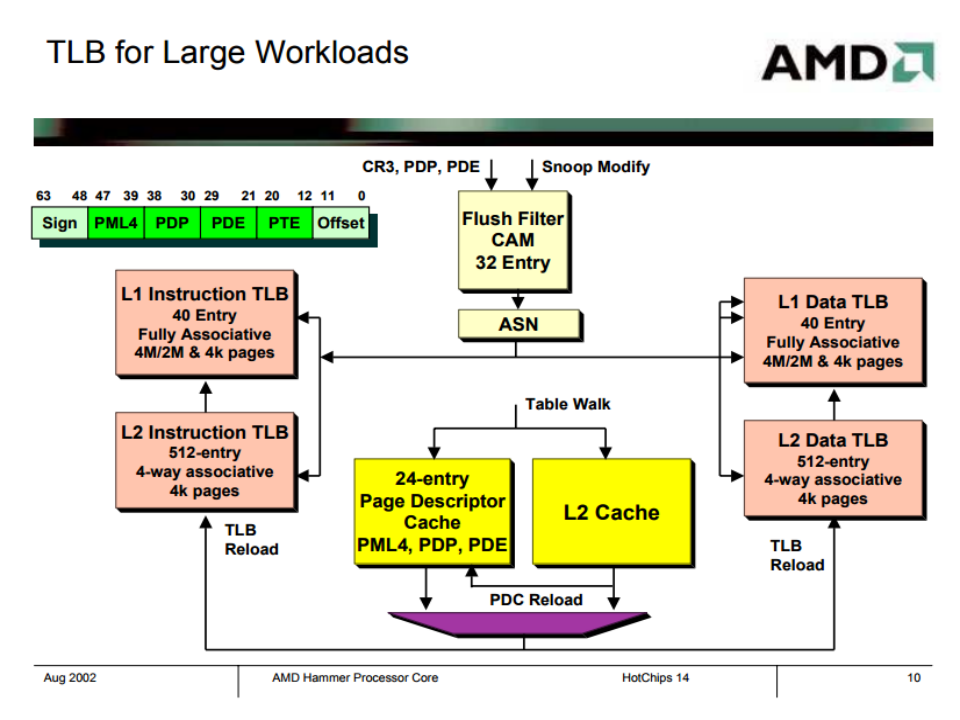
\includegraphics[scale=0.5]{figures/AMD_TLB}
\caption{AMD K8 TLB\cite{amd_ref}}
\label{fig:TLB}
\end{minipage}
\end{figure*}
\clearpage
\bibliographystyle{IEEEtran}
\bibliography{writeup}
\end{document}
